%Typeset with LaTeX
%\documentclass{owrart}
\documentclass[10pt,reqno]{amsart}
\usepackage[a4paper,margin=1.0in]{geometry}
\UseRawInputEncoding
%% -------------------------------------------------------------------------------
%% Enter additionally required packages below this comment.
\usepackage{algorithm}
\usepackage{algpseudocode}

\makeatletter
% Reinsert missing \algbackskip
\def\algbackskip{\hskip-\ALG@thistlm}
\makeatother

\usepackage{graphicx}
\usepackage{subcaption}

\usepackage{tikz}
\usepackage{amsmath}
\usepackage{mathtools}
%\usepackage[a4paper]{geometry}
%\usepackage{amsfonts}
\usepackage{amssymb}
\usepackage{amsthm}
\usepackage{mathrsfs}
\usepackage{bm}
\usepackage{algpseudocode}
\usepackage{upgreek}
\usepackage{subcaption}
% \usepackage{showkeys} %%%%%%%%%
% \usepackage{amscd}
% \usepackage{latexsym}
% \usepackage{nicefrac} 3
% \usepackage{cite}
 %\usepackage{epic}
% \usepackage{eepic}
% \usepackage{fancybox}
\newcommand{\bsnul}{{\boldsymbol 0}}
\newcommand{\cNN}{{\mathcal {NN}}}

\usepackage{graphicx}
\usepackage{epstopdf}

\mathtoolsset{showonlyrefs}

%\usepackage{epstopdf}
%\usepackage{graphicx} 

%\usepackage[pdf]{pstricks}

\usepackage[shortlabels]{enumitem}
%Standard operator
\newcommand{\abs}[1]{\lvert #1\rvert}
\newcommand{\supp}{Peratorname{supp}}
\newcommand{\grad}{{\mathbf{grad}}}
\newcommand{\curl}{\normalfont{\text{curl}}}
\newcommand{\Log}{\text{Log}}
\newcommand{\cc}{{\normalfont{\text{c}}}}
\newcommand{\loc}{{\normalfont{\text{loc}}}}

\DeclareMathOperator*{\argmax}{arg\,max}
\DeclareMathOperator*{\argmin}{arg\,min}

% Package for colors
\usepackage{xcolor}
\definecolor{ao}{rgb}{0.0, 0.5, 0.0}

%Edit colors
\newcommand{\CS}[1]{{\color{magenta}{#1}}}
\newcommand{\ra}[1]{{\color{blue}{#1}}}
\newcommand{\fh}[1]{{\color{cyan}{#1}}}
\newcommand{\todo}[1]{{\color{red}[#1]}}

\newcommand{\com}[1]{{\color{red} [#1]}}

%\usepackage{fancyhdr}
%\usepackage{datetime}
%
%\fancyhf{}
%\fancyfoot[L]{\fontsize{10}{12} \today \ \currenttime}
%\pagestyle{fancy} \usepackage{tikz}

\DeclareSymbolFont{extraup}{U}{zavm}{m}{n}
\DeclareMathSymbol{\varheart}{\mathalpha}{extraup}{86}
\DeclareMathSymbol{\vardiamond}{\mathalpha}{extraup}{87}

\usepackage{chngcntr}
\counterwithout{equation}{subsection}
\counterwithout{equation}{section} 

\usepackage{tikz}

\newcommand\encircle[1]{%
  \tikz[baseline=(X.base)] 
    \node (X) [draw, shape=circle, inner sep=0] {\strut #1};}

\usepackage{pifont}

\usepackage{fancyhdr}
\usepackage[us,12hr]{datetime} % `us' makes \today behave as usual in TeX/LaTeX
\fancypagestyle{plain}{
\fancyhf{}
\rhead{\footnotesize Version of \today}
\lhead{\thepage}
\renewcommand{\headrulewidth}{0pt}}
\pagestyle{plain}

\usepackage{color}
\newcommand{\half}{\frac{1}{2}}

\newcommand{\norm}[1]{\left \lVert #1 \right \rVert}
\newcommand{\snorm}[1]{\left \lvert #1 \right \rvert}

%fields, mathbb operators
\newcommand{\IR}{\mathbb{R}}
\newcommand{\IC}{\mathbb{C}}
\newcommand{\IZ}{\mathbb{Z}}
\newcommand{\IQ}{\mathbb{Q}}
\newcommand{\IN}{\mathbb{N}}
\newcommand{\IT}{\mathbb{T}}

% Boundary Integral Operators
\newcommand{\OV}{\mathsf{V}}
\newcommand{\OK}{\mathsf{K}}
\newcommand{\OW}{\mathsf{W}}
% 

%
%\DeclareMathOperator*{\argmax}{arg\,max}
%\DeclareMathOperator*{\argmin}{arg\,min}

\newcommand{\OA}{\mathsf{A}}
\newcommand{\Id}{\mathsf{Id}}
\newcommand{{\D}}{\normalfont{\text{D}}}
\newcommand{{\G}}{\normalfont{\text{G}}}
\newcommand{{\U}}{\normalfont{\text{U}}}
\newcommand{{\I}}{\normalfont{\text{I}}}
\newcommand{{\per}}{\normalfont{\text{per}}}
\newcommand{{\y}}{{\boldsymbol{{y}}}}
\newcommand{\Of}{\mathsf{f}}

\newcommand{{\bc}}{{\bf c}}
\newcommand{{\bx}}{{\bf x}}
\newcommand{{\by}}{{\bf y}}
\newcommand{{\bz}}{{\bf z}}
\newcommand{{\bd}}{{\bf d}}
\renewcommand{\d}{\!\!\operatorname{d}}

% Traces
\newcommand{\traced}{\gamma_{\text{D}}}
\newcommand{\tracen}{\gamma_{\text{N}}}
\newcommand{\dual}[2]{\left \langle #1,#2 \right \rangle}
\newcommand{\dotp}[2]{\left ( #1,#2 \right )}

% Matrix trace
\newcommand{\tr}[1]{\text{tr}\left ( #1 \right )}

\newtheorem{theorem}{Theorem}[section]
\newtheorem{corollary}[theorem]{Corollary}
\newtheorem{lemma}[theorem]{Lemma}
\newtheorem{prob}[theorem]{Problem}
\newtheorem{definition}[theorem]{Definition}
\newtheorem{assumption}[theorem]{Assumption}
\newtheorem{proposition}[theorem]{Proposition}
\newtheorem{example}[theorem]{Example}
\newtheorem{problem}[theorem]{Problem}

\theoremstyle{remark}
\newtheorem{remark}{Remark}
%\newtheorem{assumption}[remark]{Assumption}
%\newtheorem{example}[remark]{Example}
%\newtheorem{problem}[thm]{Problem}


%\numberwithin{equation}{section}

\begin{document}
%\begin{talk}
%
%---------
% TITLE
%---------
%

\title{Exercise Set 2 \\ 
MATH-459--Numerical Methods for Conservation Laws \\  
Autumn Semester 2021
}

\author{Professor: Martin W. Licht \\ Assistant: Fernando Henriquez B.} 

\maketitle

\subsection*{Problem 1: Method of Characteristics}

\begin{itemize}
\item[(i)] Consider the conservation law 
\begin{align}
	\frac{\partial u}{\partial t}
	-
	x
	\frac{\partial u}{\partial x}
	= 0
\end{align}
with initial value
\begin{align}
	u(x,0)=x.
\end{align}
Sketch the characteristics up to time $t=1$. Describe the graph of the function $u(\cdot,t)$
as $t$ increases.
\item[(ii)] Consider the conservation law
\begin{align}
	\frac{\partial u}{\partial t}
	+
	x
	\frac{\partial u}{\partial x}
	= 0
\end{align}
with initial value
\begin{align}
	u(x,0)=x.
\end{align}
Draw the characteristics and describe the graph of the function $u(\cdot,t)$ as $t$ increases.
\end{itemize}

\subsection*{Solution}
We start by tacking (i).
Firstly, we set $F(t,x,z) = u(x,t) -z$, hence the solution
of the conservation law
\begin{align}\label{eq:cons:law}
	\frac{\partial u}{\partial t}
	-
	x
	\frac{\partial u}{\partial x}
	= 0
\end{align}
can be understood as the surface implicitly defined as $F(t,x,z) = 0$.
Observe that \ref{eq:cons:law} can be written as
\begin{align}
	\begin{pmatrix}
		\frac{\partial u}{\partial t} \\
		\frac{\partial u}{\partial x} \\
		-1
	\end{pmatrix}
	\cdot
	\begin{pmatrix}
	1 \\
	-x \\
	0
	\end{pmatrix}
	= 0.
\end{align}
The vector $(\frac{\partial u}{\partial t},\frac{\partial u}{\partial x} ,-1)^\top $
is normal to the surface $F(t,x,z) =0$, hence
$(1,-x,0)^\top$ is a tangent vector to $F(t,x,z) =0$.
Starting from a point $(0,\xi,u_0(\xi)$ we consider the characteristic curve
with speed vector $(1,-x,0)^\top$. Considering a parametrization
$(t(s),x(s),z(s))^\top$ with $s \in \IR$ of the sought curve, we enforce its tangent 
vector to match $ (1,-x,0)^\top$. In doing so, we get the following set of ODEs
describing the characteristic curve
\begin{align}
	\frac{dt(s)}{ds} =1,
	\quad
	\frac{dx(s)}{ds} =-x,
	\quad
	\text{and}
	\quad
	\frac{dz(s)}{ds} =0.
\end{align}
Considering the aforementioned initial condition, we get the following solutions
\begin{align}
	t(s) =s,
	\quad
	x(s) = \xi \exp(-s),
	\quad
	\text{and}
	\quad
	z(s) = u_0(\xi).
\end{align}
We remark at this point that the parameters $s$ it is 
actually equal to the temporal variable $t$, and that
the solution $u(x,t)$ is constant along the characteristics
and equal to the initial condition. 
From the implicit definition of the solution of the conservation law
as $F(t,x,z) =0$, we get that 
\begin{align}\label{eq:cons:law_sol}
	u(x,t) = u_0(\xi) = u_0(x \exp(t)) = x \exp(t).
\end{align}
It is straightforward to verify that $u(x,t)$ in \eqref{eq:cons:law_sol}
is actually a solution of \eqref{eq:cons:law} in the classical sense. 
For any $\xi \in \IR$, the characteristics in the $x-t$ plane are given by
\begin{align}
	t(x)
	=
	-
	\log
	\left(
		\frac{x}{\xi}
	\right),
	\quad
	\text{for}
	\quad
	x \xi>0.
\end{align}
We proceed to tackle (ii).
As in the previous case, we consider a parametrization
$(t(s),x(s),z(s))^\top$ with $s \in \IR$ of the sought curve, we enforce its tangent 
vector to match $ (1,x,0)^\top$. We get the following set of ODEs
describing the characteristic curve
\begin{align}
	\frac{dt(s)}{ds} =1,
	\quad
	\frac{dx(s)}{ds} =x,
	\quad
	\text{and}
	\quad
	\frac{dz(s)}{ds} =0.
\end{align}
The solution to the ODEs are
\begin{align}
	t(s) =s,
	\quad
	x(s) = \xi \exp(s),
	\quad
	\text{and}
	\quad
	z(s) = u_0(\xi).
\end{align}
Again, the parameter $s$ it is 
actually equal to the temporal variable $t$, and
the solution $u(x,t)$ is constant along the characteristics.
From the implicit definition of the solution of the conservation law
as $F(t,x,z) =0$, we get that 
\begin{align}\label{eq:cons:law_sol_2}
	u(x,t) = u_0(\xi) = u_0(x \exp(-t)) = x \exp(-t).
\end{align}
It is straightforward to verify that $u(x,t)$ in \eqref{eq:cons:law_sol_2}
solves
\begin{align}
	\frac{\partial u}{\partial t}
	+
	x
	\frac{\partial u}{\partial x}
	= 0.
\end{align}
For any $\xi \in \IR$, the characteristics in the $x-t$ plane are given by
\begin{align}
	t(x)
	=
	\log
	\left(
		\frac{x}{\xi}
	\right),
	\quad
	\text{for}
	\quad
	x \xi>0.
\end{align}
\subsection*{Problem 2: Weak Solutions}

Show that a weak solution to the linear transport equation 
$$
	\frac{\partial u}{\partial t} 
	+ 
	a 
	\frac{\partial u}{\partial x}  = 0, 
$$
with $a\in \IR$ and initial data 
\begin{align}
	u(x,0) = 
	\left\{
	\begin{array}{ll}
	1, & \text{for} \quad x<0,\\
	0, &\text{for} \quad x > 0,
	\end{array}
	\right.
\end{align}
is given by
\begin{align} 
	u(x,t) = 
	\left\{
	\begin{array}{ll}
	1, & \text{for} \quad x<at,\\
	0, & \text{for} \quad x > at,
	\end{array}
	\right.
\end{align}
\subsection*{Solution}
We need to prove that for all test functions $\phi \in C^1(\IR \times [0,\infty))$
with compact support, it holds 
\begin{align}
	\int\limits_{0}^{\infty}
	\int\limits_{-\infty}^{\infty}
	\left(
		\frac{\partial \phi}{\partial t}
		u
		+
		\frac{\partial \phi}{\partial x}
		f(u)
	\right)
	\text{d}x \text{d} t
	=
	-
	\int\limits_{-\infty}^{\infty}
	\phi(x,0) u(x,0)
	\text{d}x,
\end{align}
where $f(u) = au$ in the case of this exercise.
Assume without loss of generality that $a>0$.
Then we calculate 
\begin{align}
	\int\limits_{0}^{\infty}
	\int\limits_{-\infty}^{\infty}
	\frac{\partial \phi}{\partial t}
	u \,
	\text{d}x \text{d} t
	=
	\int\limits_{-\infty}^{0}
	\int\limits_{0}^{\infty}
	\frac{\partial \phi}{\partial t}
	\text{d}t \text{d} x
	+
	\int\limits_{0}^{\infty}
	\int\limits_{x/a}^{\infty}
	\frac{\partial \phi}{\partial t}
	\text{d}t \text{d} x
	=
	-
	\int\limits_{-\infty}^{0}
	\phi(x,0)
	\text{d} x
	-
	\int\limits_{0}^{\infty}
	\phi
	\left(x,\frac{x}{a}\right)
	\text{d} x,
\end{align}
and
\begin{align}
	\int\limits_{0}^{\infty}
	\int\limits_{-\infty}^{\infty}
	\frac{\partial \phi}{\partial x}
	f(u)
	\text{d}x \text{d} t
	=
	a
	\int\limits_{0}^{\infty}
	\int\limits_{-\infty}^{at}
	\frac{\partial \phi}{\partial x}
	\text{d}x \text{d} t
	=
	a
	\int\limits_{0}^{\infty}
	\phi
	\left(at,t\right)
	\text{d}t
\end{align}
Observing that
\begin{align}
	a
	\int\limits_{0}^{\infty}
	\phi
	\left(at,t\right)
	\text{d}t
	=
	\int\limits_{0}^{\infty}
	\phi
	\left(x,\frac{x}{a}\right)
	\text{d} x,
\end{align}
and that
\begin{align}
	\int\limits_{-\infty}^{0}
	\phi(x,0)
	\text{d} x
	=
	\int\limits_{-\infty}^{\infty}
	\phi(x,0)
	u(x,0)
	\text{d} x,
\end{align}
we conclude the desired result.
\subsection*{Problem 3: Rarefaction Waves}
Consider the initial value problem 
\begin{align}
	\frac{\partial u}{\partial t}
	+
	\frac{\partial f(u)}{\partial x}
	=0,
	\quad
	u(x,0) = u_0(x),
\end{align}
with $f(u) =\frac{u^2}{2}$, and
\begin{align}\label{eq:initial_condition}
	u_0(x)
	=
	\left \{
	\begin{array}{ll}
	2, \quad0<x<1, \\
	0, \quad\text{otherwise},
	\end{array}
	\right.
\end{align}
Here a rarefaction wave arises at one discontinuity and a shock at the other. 
The goal of this exercise is to determine the exact solution for all $t>0$. 
In this setup, the rarefaction wave catches up with the shock at some time $T_c>0$.
\begin{itemize}
	\item[(i)]
	Draw the profile of $u_0(x)$
	and sketch the characteristics in the strip 
	$0 < t < T_c$ of the $x-t$ plane.
	\item[(ii)]
	Determine the exact solution for $0 < t < T_c$.
	\item[(iii)]
	Let $x_s(t)$ be shock's location at $t > T_c$. 
	By using the Rankine-Hugoniot jump condition construct an ODE to determine 
	$x_s(t)$ for all $t > T_c$. 
	In the sketch you drew in (i), extend the characteristic lines to $t > T_c$.
\end{itemize}

\subsection*{Solution}

\begin{figure}
    \centering
    \begin{subfigure}[b]{0.5\textwidth}
        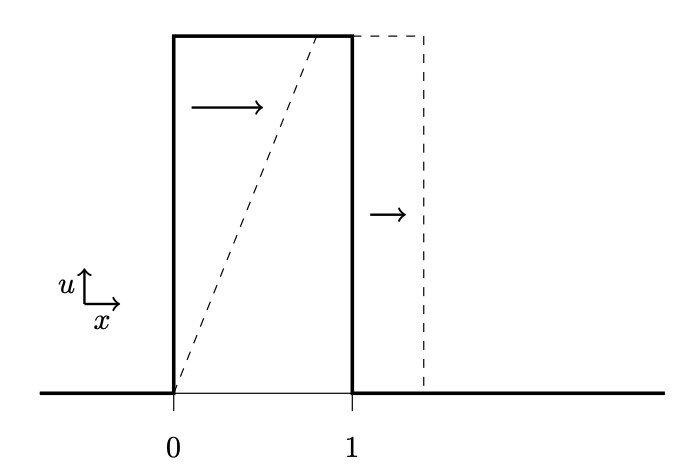
\includegraphics[width=\textwidth]{Figs/ex_set_2_3}
        \caption{Initial data $u_0$, given by \eqref{eq:initial_condition}.
        The rarefaction wave and the shock both move in the positive direction.}
        \label{fig:u_0}
    \end{subfigure}
    ~
    \begin{subfigure}[b]{0.5\textwidth}
        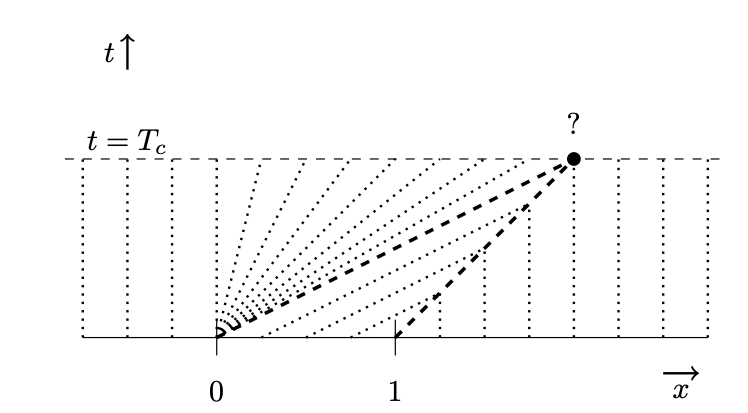
\includegraphics[width=\textwidth]{Figs/ex_set_2_2}
        \caption{Characteristics of the solution of the Burger's equation
        up until time $T_c$. The rarefaction wave moves faster than
        the shock and at some point in time $t = T_c > 0$ they meet,
        and the characteristics cross each other.}
        \label{fig:characteritics}
    \end{subfigure}
    \caption{Initial condition $u_0$ and characteristics up until $T_c$.}
    \label{problem3_part1}
\end{figure}

\begin{itemize}
\item[(a)]
Figure \ref{problem3_part1} contains a sketch of the initial data profile
$u_0$ with characteristics evolving. To determine
the speed of the shock originating at $x = 1$, we use the Rankine-Hugoniot jump condition
$$
s_{shock}=\frac{f\left(u_{l}\right)-f\left(u_{r}\right)}{u_{l}-u_{r}}=\frac{\frac{1}{2} 2^{2}-\frac{1}{2}(0)^{2}}{2-(0)}=1.
$$
At the discontinuity at $x = 0$ we expect a rarefaction wave to arise. 
From the general solution to the rarefaction wave, we have that the
right front of this wave moves with a speed of $s_{rf} = f′(u_r) = 2$.
The rarefaction wave thus moves to the right twice as fast as the
shock wave and at some point in time the waves must meet.
\item[(b)]
First we seek to determine the exact solution for $0<t<T_{c}$, where $T_{c}$ is the time when the rarefaction wave catches up with the shock. The time $T_{c}$ is trivial to find: Since the position of the rarefaction front is $x_{r f}=2 t$ and the position of the shock is $x_{\text {shock }}=t+1$, we have $T_{c}+1=2 T_{c}$, namely $T_{c}=1 .$ Thus,
$$
u(x, t)=\left\{\begin{array}{ll}
0 & x<0 \\
\frac{x}{t} & 0<x<2 t \\
2 & 2 t<x<t+1 \\
0 & t+1<x
\end{array}\right.
$$
$$
s_{s h o c k}=\frac{f\left(u_{l}\right)-f\left(u_{r}\right)}{u_{l}-u_{r}}=\frac{\frac{1}{2} 2^{2}-\frac{1}{2}(0)^{2}}{2-(0)}=1
$$
\item[(c)]
What happens at $t>T_{c} ?$ We again use the Rankine-Hugoniot jump condition, now to construct an $\mathrm{ODE}$ for the position of the shock $x_{s}$ after the rarefaction and shock wave have merged:
$$
\frac{d x_{s}(t)}{d t}=\frac{f\left(u_{l}\right)-f\left(u_{r}\right)}{u_{l}-u_{r}}=\frac{\frac{1}{2}\left(\frac{x_{s}(t)}{t}\right)^{2}-\frac{1}{2}(0)^{2}}{\frac{x_{s}(t)}{t}-(0)}=\frac{1}{2} \frac{x_{s}(t)}{t}
$$
This ODE has the general solution $x_{s}(t)=C \sqrt{t}$. At $t=1$ we know that $x_{s}=2$ so $C=2$. But what about the profile of $u(x, t) ?$ For times $t>T_{c}$, we expect the solution to the left of the shock-curve to be obtained from the rarefaction solution, i.e., $u=x / t$, while the solution on the right to be $u=0$. Note that this is compatible with the entropy condition for a shock. Thus, the solution can be expressed as
$$
u(x, t)=\left\{\begin{array}{ll}
0 & x<0 \\
\frac{x}{t} & 0<x<2 \sqrt{t} \\
0 & x>2 \sqrt{t}
\end{array}\right.
$$
Figure \ref{problem3_part2} shows the characteristic curves in the $x-t$ plane up to $t=T_{c}$ and beyond. One can see that the information originating from $(x, t)=(0,0)$ reaches up to the shock, even after the rarefaction front have caught up with it. This means that for $t>T_{c}$, in $0<x<x_{s}$, the solution is determined exclusively by the rarefaction wave, and is not affected by the location, or the existence of the shock.

\begin{figure}
    \centering
    \begin{subfigure}[b]{0.5\textwidth}
        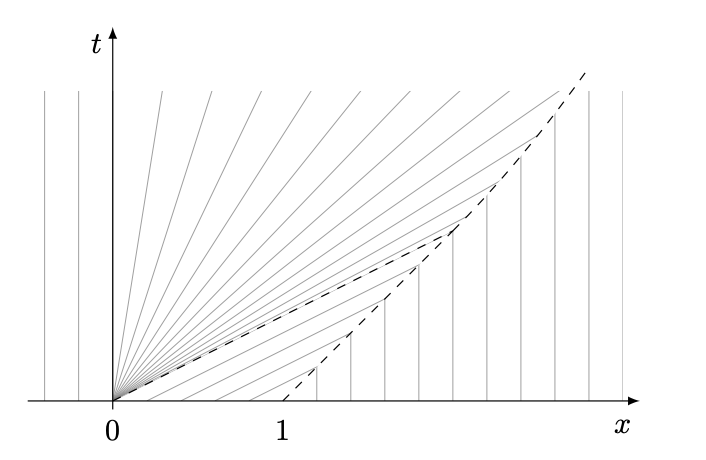
\includegraphics[width=\textwidth]{Figs/ex_set_2_4}
%        \caption{Initial data $u_0$, given by \eqref{eq:initial_condition}.
%        The rarefaction wave and the shock both move in the positive direction.}
%        \label{fig:u_0}
    \end{subfigure}
    \caption{The characteristic curves (gray lines) of u in the $x-t$ plane.}
    \label{problem3_part2}
\end{figure}
\end{itemize}

%\begin{figure}[t!]
%    \centering
%    \begin{subfigure}[t]{0.5\textwidth}
%        \centering
%        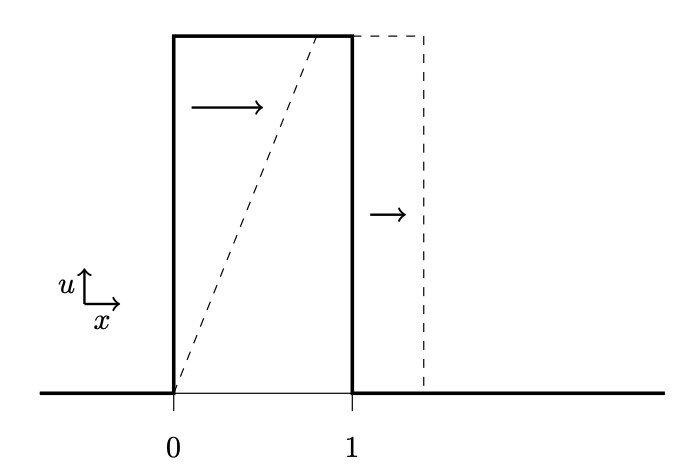
\includegraphics[height=2.5in]{Figs/ex_set_2_3}
%        \caption{a}
%        \label{subfig:loss_alg_2}
%    \end{subfigure}%
%    \\
%    \begin{subfigure}[t]{0.5\textwidth}
%        \centering
%        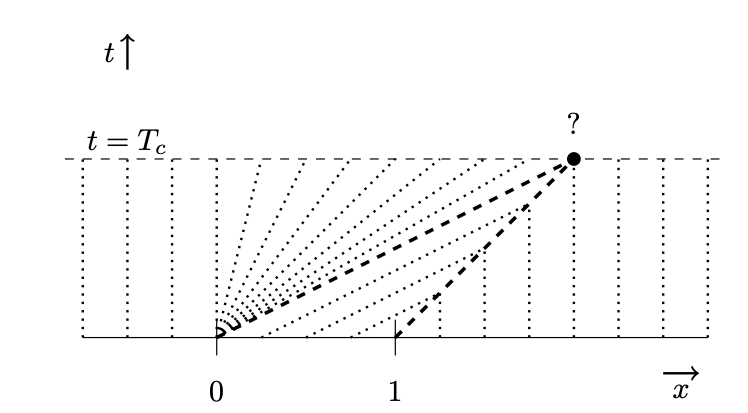
\includegraphics[height=2.5in]{Figs/ex_set_2_2}
%        \caption{a}
%        \label{subfig:error_alg_2}
%    \end{subfigure}
%    \caption{a}
%}
%\label{fig:alg_2}
%\end{figure}

%\begin{figure}[h!]
%\centering
%\begin{tikzpicture}[scale=1]
%\draw (0,0) -- (2, 2);
%\end{tikzpicture}

%\caption{Characte}
%\label{fig:L_domain}
%\end{figure}
\bibliography{ref}{}
\bibliographystyle{plain}
\end{document}
